\documentclass{article}
\bibliographystyle{unsrt}
\usepackage{amssymb,mathtools,graphicx,algorithm,amsmath,algpseudocode,hyperref}
\usepackage[margin=1in]{geometry}
\begin{document}

\title{Maximum Flow\\Comparative Analysis of Ford-Fulkerson and Edmonds-Karp}

\author{Pedro Rodriguez\\
University of Colorado at Boulder
}

\maketitle
\section{Introduction}
The first research into network flow algorithms began in the early and mid 20th century. Initial research by A.N. Tolstoi sought to optimize production networks such as railroads in the Soviet Union\cite{Schrijver:2002dj}. The subject later picked up interest amongst the American scientists Ford and Fulkerson who devised the first known algorithm for computing the maximum flow through a network\cite{Ford:1956vc}. 

The maximum flow problem is defined by: Finding the maximum flow through a network from a source vertex $s$ to a sink vertex $t$ in a directed graph $G$ which has edges labeled with flow capacities.

Twenty years after Ford-Fulkerson published their results Edmonds and Karp independently improved upon the algorithm by replacing the depth-first search strategy used in Fork-Fulkerson with breadth-first search\cite{Edmonds:1972ht}. This change improved the algorithmic efficiency from $O(E|f|)$ where $f$ is the maximum flow to $O(VE^2)$. This idea was further improved upon by Dinic's who exploited the property that the flow paths were monotonically increasing to achieve an even better $O(V^2E)$ running time\cite{Dinic:lsM40ti7}. All of these algorithms share a common strategy: find an augmenting path from $s$ to $t$ to push flow across and repeat until there is no such path. At this point the algorithm terminates and returns the maximum flow value and paths.

Beyond the natural applications of maximum flow algorithms to optimizing supply chains, routing, and others it has gained popularity as a sub-algorithm call in more advanced problems. For example, it was recently used to solve the k-clique densest subgraph problem\cite{tsourakakis2015k}, and various computer vision such as object category segmentation, image deconvolution, super resolution, texture restoration, character completion, and 3D segmentation\cite{Verma:2012gs}. It has also been used to solve other problems such as minimum path cover in directed acyclic graphs, maximum cardinality bipartite matching, and in the "real-world" baseball elimination, airline scheduling, and circulation-demand\cite{wiki:maxflow}.

\section{Problem Statement}
\subsection{Formal Problem Statement}
\label{formal-problem-statement}
Now we proceed to formally defining the maximum flow problem. The problem is defined as given a graph with: 
\begin{enumerate}
	\item Vertex set $V$
	\item Directed edge set $E$
	\item Source vertex $s\in V$ such that no edges are incident
	\item Sink vertex $t\in V$ such that no edges leave it
	\item Integer edge capacities $c_{uv}\in \mathbb{R}_{\ge 0}, \forall (u,v)\in E$
\end{enumerate}

And subject to the conditions:
\begin{enumerate}
	\item $f_{uv}\coloneqq$ variable indicating flow from $u$ to $v$
	\item  $f_{uv}\le c_{uv},\forall (u,v)\in E$
	\item $\forall v\in V\text{ such that }v\ne s,t:\sum_{(u,v)\in E}f_{uv}=\sum_{(v, u)\in E} f_{vu}$
\end{enumerate}

Find the flow assignments $f_{uv}$ such that network flow $|f|\coloneqq\sum_{(s,v)\in E}f_{sv}$ is maximized.

\subsection{Graphical Depiction}
To fix ideas we will continue by describing a concrete instance of the problem. For example, consider the example in figure \ref{simple-flow}\cite{wiki:fordfulk}. In the figure, each edge is labeled by a pair of numbers which are presented as $f_{uv}/c_{uv}$. This represents how much flow $f_{uv}$ is passing through an edge with capacity $c_{uv}$. By inspection, it is easy to deduce that the maximum flow is $2000$ with $1000$ flowing through the top and $1000$ flowing through the bottom. This representation makes the meaning of the conditions (1) and (2) clear. Condition (3) expresses that the flow into any vertex which is not a source or sink must be the flow out of that vertex. Finally, the objective can be explained by noting (with proof later) that the maximum flow from $A$ to $D$ is equivalent to taking a cut across $A$.

Before moving on, lets consider a simple algorithm: find a path through the network and push the maximum possible flow through until pushing flow is impossible. One can see this may result in the optimal solution, but if one path found is the one cross $BC$, then the optimal flow will never be found. This hints that the simple graph construction is insufficient to solve the maximum flow problem.

\begin{figure}[!ht]
	\caption{Simple flow network}
	\centering
	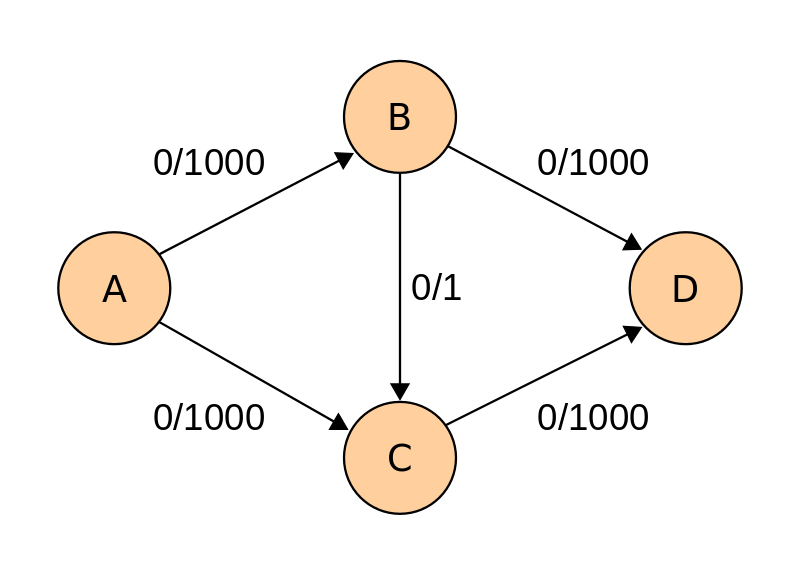
\includegraphics[width=0.5\textwidth]{images/simple-flow.png}
	\label{simple-flow}
\end{figure}

\section{Algorithm Analysis}
In this section we will first present the very similar Ford-Fulkerson and Edmonds-Karp algorithms, prove their correctness, and analyze their asymptotic behavior in both time and space complexity.

\subsection{Algorithm}
Before proceeding to the algorithm itself, we must make a few additional definitions and constructions. First we will define a $G_f(V,E_f)$ which we will call the residual graph. In this graph, the capacities are defined as $c^f_{uv}=c_{uv}-f_{uv}$ and there is zero flow. We additionally define that $\forall (u,v)\in E,\ f_{uv}=-f_{vu}$. Combining these two loosens the constraints from the original graph to allow cases where if $f_{uv}>0$ and $c_{uv}=0$ that $c^f_{vu}=c_{vu}-f_{vu}=f_{uv}>0$. As will be proven, this allows for algorithm to function correctly. We now proceed to stating the main algorithm as Algorithm \ref{ff-ek-algorithm}.

\begin{algorithm}
\label{ff-ek-algorithm}
\caption{Ford-Fulkerson and Edmonds-Karp}
\begin{algorithmic}[1]
\Function{max\_flow(G,c,s,t)}{}
\State Input: $G,c,s,t$ as described in \ref{formal-problem-statement}
\State Output: Flow $f_{max}$ and paths to achieve it
\Loop
\State $path\gets augmenting\_path(G_f,s,t)$
\If {$path = None$}
\State break
\EndIf
\State $f_{min}=\min_{(u,v)\in path} c^f_{uv}$
\For{$(u,v)\in path$}
\State $f_{uv}\gets f_{uv}+f_{min}$
\State $f_{vu}\gets f_{vu}-f_{min}$
\EndFor
\EndLoop
\State $f_{max}\gets \sum_{(s,v)\in E}f_{sv}$
\State $paths\gets$ paths/flows from $s$ to $t$ in created graph
\State \Return $f_{max},paths$
\EndFunction
\end{algorithmic}
\end{algorithm}

The algorithm proceeds in two alternating phases: finding an augmenting path from $s$ to $t$ in $G_f$ and pushing the maximal viable flow across that path. When an augmenting path cannot be found, then the algorithm terminates and returns the current maximal flow.

We define an augmenting path as any path from $s$ to $t$ in $G_f$ such that $c^f_{uv}>0\ \forall (u,v)\in path$. The algorithm was not previously specified because its definition determines whether the algorithm is known as Ford-Fulkerson or Edmonds-Karp. If the augmenting path is found using depth first search then the algorithm is called Fork-Fulkerson. If the augmenting path is found using breadth first search then the algorithm is called Edmonds-Karp. With that in mind, we now define the two possible augmenting path algorithms. Note that the $0th$ element of a list is considered the back and the last element of a list is considered the front. Additionally the notation $vec[a;b]$ is short for creating a vector of length $b$ with values initialized to $a$.

\begin{algorithm}
\label{ap-algorithm}
\caption{Augmenting Path Algorithm}
\begin{algorithmic}[1]
\Function{augmenting\_path($G_f$, s, t, search)}{}
\State $V, E_f\gets G_f$
\State $search\_list \gets list()$
\If {$search = BFS$}
\State $pop \gets list.pop\_front$
\State $push \gets list.push\_back$
\Else
\State $pop \gets list.pop\_front$
\State $push \gets list.push\_front$
\EndIf
\State $push(search\_list, s)$
\State $distances\gets vec[\infty; |V|]$
\State $parents\gets vec[\infty; |V|]$
\State $u\gets pop(search\_list)$
\While{$u \ne None\ and\ u\ne t$}
\For{$v$ in $neighbors(u)$}
\If{$distances[v] =\infty\ and\ c^f_{uv}>0$}
\State $distances[v]\gets distances[u] + 1$
\State $parents[v]\gets u$
\State $push(search\_list, v)$
\EndIf
\EndFor
\State $u\gets pop(search\_list)$
\EndWhile
\State\Return $u == t$, reconstruct\_path(s, t, parents)
\EndFunction
\Statex
\Function{reconstruct\_path(s, t, parents)}{}
\State $path\gets list()$
\State $node\gets t$
\Loop
\State $path.append(node)$
\If{$node == s$}
\State \textbf{break}
\EndIf
\State $path\gets parents[node]$
\EndLoop
\State\Return $reverse(path)$
\EndFunction
\end{algorithmic}
\end{algorithm}

Algorithm \ref{ap-algorithm} is essentially a breadth first search or depth first search from the source to the sink with the existence of an edge being defined as when $c^f_{uv}>0$. The output of this search is whether a path exists followed by a vector containing back pointers. This is then used to reconstruct the original path from $s$ to $t$ in $reconstruct\_path$.

Combining Algorithms \ref{ff-ek-algorithm} and \ref{ap-algorithm} yields Ford-Fulkerson when depth first search is used and Edmonds-Karp when breadth first search is used.

\subsection{Correctness}
In this section we first prove that the maximum flow algorithm is correct assuming augmenting paths is correct, then prove that the augmenting paths algorithm is correct to complete the proof.
\subsubsection{Maximum Flow}
Consider the following lemmas:
\begin{enumerate}
	\item \label{lemma:initial-flow} The initial flow through the network $f_{uv}=0,\forall (u,v)\in E$ is a valid flow since $c_{uv}$ is at least $0$ for all edges present in the graph.
	\item Since the original graph contains no parallel edges or cycles, if $c_{uv}>0$ then $c_{vu}=0$. Otherwise this would imply that a cycle would exist in the original graph which is prohibited.
	\item \label{lemma:pos-flow} Given an edge $(u,v)$ by definition $c_{uv}^f=c_{uv}-f_{uv}>0$. If $c_{uv}>0$ then an additional flow up to and including $c_{uv}^f$ can be pushed across $(u,v)$ while preserving the capacity constraint that $c_{uv}\ge f_{uv}$. This is true because the new flow $f_{uv}'=c_{uv}^f+f_{uv}=c_{uv}-f_{uv}+f_{uv}=c_{uv}$ which satisfies the capacity constraint.
	\item \label{lemma:neg-flow} Consider the case where $c_{uv}=0$. If $c_{uv}^f>0$ then $c_{uv}^f=c_{uv}-f_{uv}=-f_{uv}>0$. The maximal value of the new flow would be $f_{uv}'=c_{uv}^f+f_{uv}=c_{uv}-f_{uv}+f_{uv}=0$. This shows that for any path augmentation when $c_{uv}=0$ that flow is conserved since $f_{uv}'\le 0\le c_{uv}$
	\item \label{lemma:valid-flow} The augmented flow pushed across the path is $\min c_{uv}^f=c_{uv}-f_{uv}>0$ which implies that for the minimal flow edge $f_{uv}$ in the path, it is brought up to the full capacity $c_{uv}$. This guarantees that the flow function $f$ is valid since it does not violate the capacity constraint (flow cannot exceed capacity). Since all other edges have equal or greater capacity, then the flow function $f$ stays valid across the entire network after any flow augmentation.
	\item \label{lemma:source-zero} Consider the source edges $(u,v)\in E$ where $u=s$ and $c_{uv}=0$. Since $s$ is a source, it can have no incident edges with $c_{uv}>0$ otherwise it would be an invalid flow network. Therefore $c_{uv}^f=0$ at all times which implies that source edges with $c_{uv}=0$ will never have any flow across them.
	\item \label{lemma:increasing-flow} Consider the source edges $(u,v)\in E$ where $u=s$ and $c_{uv}>0$. Since $c_{uv}\ne 0$ by lemma \ref{lemma:pos-flow} the flow is positive. Therefore, at every iteration the flow across the source edges increases by at least $1$.
	\item \label{lemma:saturated} Define $V_s$ to be all the vertexes reachable from $s$ when the algorithm terminates. By definition, this occurs when no augmenting paths can be found which is equivalent to stating that $c_{uv}^f\ngtr 0$ for all edges from $V_s$ to $V-V_s$. This implies that for all edges across these sets that either $c_{uv}=0$ or $c_{uv}=f_{uv}$. In either case, this is equivalent to saying that all the edges are saturated.
\end{enumerate}

With these lemmas in mind, lets stitch them together for a complete proof. By lemma \ref{lemma:initial-flow} the initial zero flow is a valid flow. Lemmas \ref{lemma:pos-flow} and \ref{lemma:neg-flow} show that for any edge and its capacity, the augmented flow is a valid flow for the edge with minimal $c_{uv}^f$. By lemma \ref{lemma:valid-flow} the augmented flow is valid for the entire path, not just the minimal edge. By lemmas \ref{lemma:source-zero} and \ref{lemma:increasing-flow} the total flow across the network is increasing by at least $1$ at each iteration. Since the initial flow is valid, this proves that every iteration yields an increase in flow across the graph that creates a new valid flow. Since the maximum flow is finite and the flow increases by at least $1$ at each iteration, this proves that the algorithm terminates after at most $f_{max}$ iterations with a valid flow.

We will now show that the flow is maximal through a proof by contradiction. Suppose that the flow returned is not maximal. This would imply that there exists some path $A$ from $s$ to $t$ along which flow can still be pushed. From lemma \ref{lemma:saturated} we know that $V_s$ includes only vertexes reachable from $s$, but that cannot reach $t$. Analogously, the edges from $V_s$ to $V-V_s$ form a cut along the graph. Therefore, any path from $s$ to $t$ including $A$ must contain an edge in the cut. Since flow can be pushed from $s$ to $t$, the edge is not saturated. However, from lemma \ref{lemma:saturated} we know that all edges that are part of the cut are saturated. Since this is a contradiction, then it is impossible for any path to exist where flow can be pushed. Therefore, this proves that the flow returned is maximal.

\subsubsection{Augmenting Path}
In this section we aim to prove that the augmenting paths algorithm will return a path from $s$ to $t$ if one exists or return that one does not exist. Through a general framework, this will be proven for both breadth first search and depth first search. In algorithm \ref{ap-algorithm} we first initialize some list structure to empty. Also initialized are a distances vector and parents (backpointer) vector. When distance is $\infty$ it implies that the given vertex has not been visited. Similarly, the parent of a vertex being set to $\infty$ implies that the vertex does not have a parent in the search. The final part of the algorithm initialization is to push the source on top of the list structure.

Consider an arbitrary vertex $u$ which is pulled from the list structure. We will show that all nodes reachable from $u$ are marked as visited. In the loop, the neighbors of $v$ are fetched. Either they have already been visited, are not in the residual graph, or are processed. When a vertex is processed, it is pushed onto the list, marked as visited, and has its distance set. Consider that $|V|$ is finite, so the number of nodes that can be marked is also finite which implies that the algorithm terminates after a finite number of iterations. Note that the algorithm only terminates when the list structure is empty which can only be empty if exactly zero vertexes need to be processed (since processing a vertex adds it to the list structure). Since none of the vertexes are marked as processed anymore, they must be marked as visited.

Now by induction we will show that all the ancestors of $u$ are marked as visited. The base case considers when the $u$ from above is processed. Therefore, all of the children of $u$ are either already visited or processed. By the reasoning above, we know that eventually all the children of $u$ are processed. The inductive step will consider when the children of $u$ are processed. When they are, all their children will be marked visited or to be processed. Therefore by induction, all the ancestors of $u$ will be processed. Finally, since all vertexes are eventually processed then by elimination all the ancestors of $u$ will be marked as visited.

To complete the proof, consider when $u=s$. Since all ancestors of $s$ will be marked as visited, if $t$ is an ancestor of $s$ then it will be visited. If it is not, then it will not be found. By following the back pointers, the original path from $s$ to $t$ will be found and returned if it exists. This shows that for any list structure, the augmenting paths algorithm will return a path from $s$ to $t$ if it exists. Therefore, any augmenting path algorithm is correct and therefore the max flow algorithm is correct. The analysis of breadth first search and depth first search as augmenting path algorithms will be left to the complexity analysis sections since that is what changes between the two.

\subsection{Ford-Fulkerson Complexity}
Let the list structure in the augmenting paths algorithm is a stack. Consider the order of vertexes visited: the deepest are visited first since vertex children are put on a stack. This is precisely the definition of depth first search. When the max flow algorithm uses depth first search it is called Ford-Fulkerson.

\subsubsection{Time Complexity}
By the max flow correctness proof, we know that at each iteration flow is increased by at least $1$. This implies that the number of iterations is bounded by the maximum flow we call $f_{max}$. Depth first search in the worst case visits all vertexes and edges which is $O(|V|+|E|)$. In the worst case if there are $n$ vertexes the number of edges is $\frac{n(n-1)}{2}=O(|V|^2)$. This implies that the worst case time complexity of depth first search is $O(|E|)$. Finally, since depth first search is run maximally $f_{max}$ times the time complexity is $O(f|E|)$.

\subsubsection{Space Complexity}
The storage used by Ford-Fulkerson is defined by the size of the stack, parent pointer vector, and distances vector. The size of the parent pointer vector and distance vector is $|V|$ since there is an entry per vertex. The maximum size of the stack is all the vertexes which is $|V|$. Therefore, the overall space complexity is $O(|V|)$.

\subsection{Edmonds-Karp Complexity}
Let the list structure in the augmenting paths algorithms is a queue. Consider the order of vertexes visited: the shallowest are visited first since the vertex children are put on a queue. This is precisely the definition of breadth first search. When the max flow algorithm uses breadth first search it is called Edmonds-Karp.

\subsubsection{Time Complexity}
Now we will show that the runtime of Edmonds-Karp is $O(VE^2)$. Like with Ford-Fulkerson, the augmenting paths algorithm runtime is also $O(|V|+|E|)=O(|E|)$ so it remains to be shown that it is called $O(VE)$ times.

First, consider the levels of the graph $G_f$ to be all vertexes reachable at consecutive distances. For example, in figure \ref{simple-flow} $A$ is at level $0$ since it is reachable at $0$ distance, $B$ and $C$ are at level $1$ since they are reachable at $1$ distance, and $D$ is at level $2$ since it is reachable at $2$ distance. For any BFS path there will be exactly one vertex from each level, otherwise it wouldn't be a shortest path.

Consider a path $P$ found by breadth first search along which flow will be augmented, and the edge changes that could occur from an iteration of Edmonds-Karp. Consider an edge $(u,v)\in P$ and the changes which may occur to it. From the level definition, if the distance to $u$ is $d$ then the distance to $v$ must be $d+1$. If flow is pushed across $(u,v)$ this means that an edge is created in the opposite direction, or more precisely from distance $d+1$ to $d$. This shows that any edge added by Edmonds-Karp must be from level $d+1$ to $d$, therefore it does not decrease the distance from $s$ to $t$. Therefore the paths found from BFS are monotonically increasing.

We call edges which were minimal in $\min c_{uv}^f$ bottlenecks. We will now bound the number of times that a given bottleneck edge can be in a shortest path. Consider a bottleneck edge $(u,v)$ which by definition exist in level $d$ and $d+1$. The new edge created must point from $v$ which is at $d+1$ to $u$ which is at $d$. In order for the new bottleneck edge $(v,u)$ to show up again the level of  $v$ and $u$ must be $d$ and $d+1$, but are currently $d+1$ and $d$. Therefore, at least two iterations are needed to increase the level of $u$ from $d$ to $d+2$. Therefore, the bound on the number of times the edge $(u,v)$ or $(v,u)$ is $1/2$ the number of iterations. Note that every time a bottleneck edge appears again the path length must have increased, and the maximum path length is $|V|$. Therefore the maximum number of times that a a bottleneck edge can appear again is $|V|/2$. At each iteration at least one bottleneck edge is guaranteed to be found by the correctness proof. Since the maximum number of edges is $O(E)$ and the maximum number of iterations a given edge can appear in is $O(V)$ the total number of calls to the algorithm is $O(EV)$. Since each iteration takes $O(E)$ the total running time is $O(VE^2)$


\subsubsection{Space Complexity}
As with Ford-Fulkerson, the only data structures used in Edmonds-Karp are a list with maximal size $V$, and two vectors with length $|V|$. Therefore the space complexity is $O(V)$.

\section{Runtime}
In this section we will analyze the performance of Ford-Fulkerson and Edmonds-Karp on specific graphs which showcase the situations in which each performs badly and thus near the asymptotic bound, and perform well and thus much better than the asymptotic bound.

\subsection{Worst Case}
The pathologically worse case for Ford-Fulkerson would be to increase the flow by $1$ at each iteration. Consider the graph from \ref{simple-flow}, and suppose that depth first search returned the alternating paths $ABCD$ and $ACBD$. Since the flow across $BC$ is $1$, this would result in $O(f)$ iterations where $f=2000$. More generally, the degenerate case for Ford-Fulkerson is when paths with low $c_{uv}^f$ have low or even $1$ integer values, and get selected often or always.

This motivates the desire to have a max flow algorithm whose runtime is independent of the maximum flow. In this report we discuss Edmonds-Karp in detail which achieves this goal, but also has inputs where it performs near its asymptotic bound. This occurs when bottleneck edges re-appear from the breadth first search the maximum number of times $|V|$. To get a glimpse at this case consider the graph in figure \ref{ek-flow}. Suppose that the first path found is $suvt$ along which $5$ flow is pushed. It should be obvious that the optimal would be to reserve $v$ for the flow comping from $a$. This however cannot occur until flow is pushed along $sueft$ and $sacdt$ since they are shortest paths. In order to fix the flow path $suvacdt$ needs to be chosen which would occur after two iterations at which time the flow could finally be fixed to optimal

\begin{figure}[!ht]
	\caption{Edmonds Karp Worst Case}
	\centering
	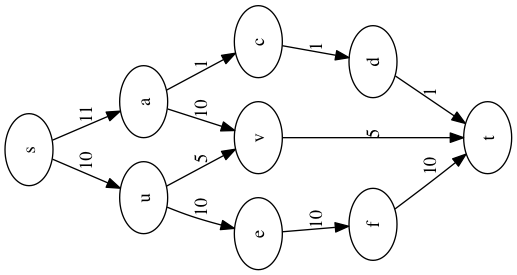
\includegraphics[width=0.5\textwidth]{images/edmonds-karp.png}
	\label{ek-flow}
\end{figure}

\subsection{Average Case}
The performance of both algorithms is highly dependent on the input graph structure which makes characterizing an average case difficult or impossible. Additionally, artifacts of common implementations (including this one), can cause widely varying performance. For example, in Ford-Fulkerson the ordering of edges in the depth first search can lead to widely varying behavior, but can be addressed by randomization methods \cite{graph-paths}. For these reasons it is not reasonable to report an average case since it is so dependent on input and specific implementation.

\subsection{Best Case}
The best case performance for both of these algorithms is when the minimum number of iterations occur. The trivial case for both graphs is that a single flow push results in termination of the algorithm. In both of these algorithms, as the number of times a single edge appears in the augmenting path decreases the better performing it becomes up to $O(E)$ for Ford-Fulkerson and $O(E)$ for Edmonds-Karp.

\section{Experiments}
The experiments in the following section were performed with the code attached to this project which is also available at \url{https://github.com/EntilZha/max_flow}. The source code for Ford-Fulkerson and Edmonds-Karp can be found in the "src/lib.rs", the running harness in "src/bin.rs", and various python and bash scripts used for formatting input data in the root directory. The algorithms were implemented using the Rust programming language version 1.8 \cite{rust}. All experiments were run on Amazon Web Services Elastic Cloud Compute with m4.2xlarge instances which have 8 2.4GHz Intel Xeon CPU cores and 32GB of memory\cite{aws}. Data sets used either the DIMACS format or an adjacency list representation\cite{dimacs}.

\subsection{Random Input Generation}
For testing, a randomized flow graph generator was created. Since the flow algorithm is highly sensitive to the graph structure, it is not representative for all inputs, but it is sufficient to verify asymptotic correctness. As input the generator takes an integer $l$ representing number of layers, integer $k$ representing layer size, $f$ the maximum flow through an edge, and interconnect ratio $r\ge 1$. The output will be a graph which has $l$ layers, and each layer having $k$ vertexes. Between layer $i$ and layer $i+1$, $k$ edges with $f$ flow are added such that the two layers form a bipartite graph with all nodes connected. Following this, edges are randomly added between layer $i$ and $i+1$ until $\lfloor r\cdot k\rfloor\le |E_{i,i+1}|$ where $E_{i,i+1}$ are the edges going from layer $i$ to layer $i+1$. The flow across these edges are sampled uniformly from $[1,f]$. All the layers were connected in this fashion while the first and last layers were fully connected to a source $s$ and sink $t$ with all edges having randomized flow like above. The experiments in the following section vary $l$ and $k$ while running $r,f$ through a wide range of values. The result of this generation process is a many layers of bipartite graphs with a randomized distribution of edges, but an easily verifiable maximum flow.

\subsection{Scaling}
To test these algorithms $f=100$, and $l,k,r$ varied. For each pair of values $(l,k)$ $r$ ranged from $1$ to $100$ by $10$ with each experiment being repeated five times. In these experiments $l=k$ for values of $50,100,150,220$. The cap value of $220$ was chosen since this resulted in 20GB/32GB of memory being used. In total this resulted in $4\cdot 10\cdot 5=200$ experimental results for each of Ford-Fulkerson and Edmonds-Karp (400 total). In terms of $|V|$, $|E|$, and $f$, the input size ranged from $|V|=2500$ to $|V|=48400$, $|E|=5100$ to $|E|=8866000$, and $f=~3500$ to $f=25000$. It should be clear that these values provide a more than adequate range of values to test against since they span many orders of magnitude in the absolute sense, but in the total asymptotic runtime as well since they are $O(f|E|)$ and $O(E^2V)$.

\subsubsection{Ford-Fulkerson}
Now we proceed to analyzing the asymptotic performance of Ford-Fulkerson by considering figure \ref{ff-performance}.

\begin{figure}[!ht]
	\caption{Ford-Fulkerson Performance}
	\centering
	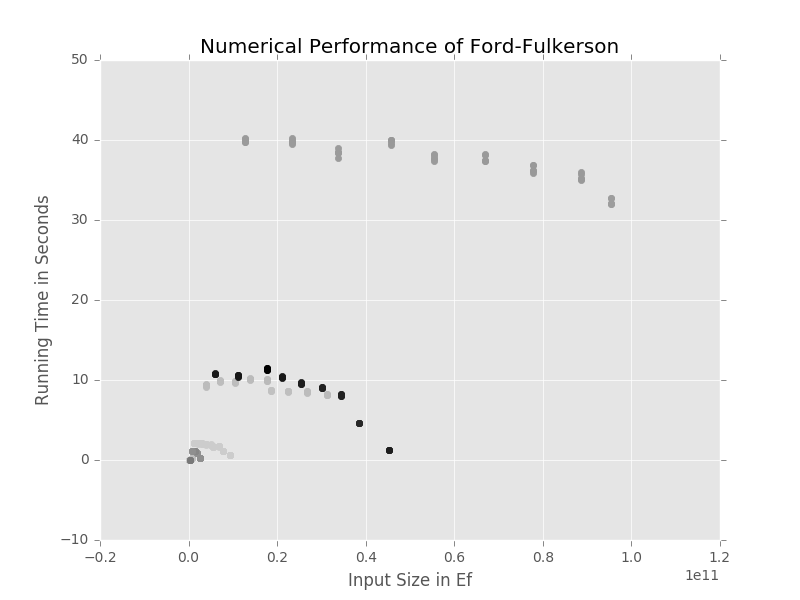
\includegraphics[width=0.5\textwidth]{images/ff-performance.png}
	\label{ff-performance}
\end{figure}

This figure plots $Ef$ versus the algorithm running time with the increasing blackness of circles indicating the experiments that achieved the highest maximum flow across all experiments. Since the algorithm is $O(Ef)$ one would expect that the runtime plot as a function of these variables should be a linear function since the asymptotic order only allows it to vary by some constant. Figure \ref{ff-performance} clearly shows a linear relationship which is verified by linear regression with good statistical values of $r=.738,r^2=.54$. One can also see that as the graph and flow increases so does the spread of the data points. This can be attributed to the fact that there is high variance in the impact of $f$ in the runtime depending on the specific graph structure. These results indicate that this implementation of Ford-Fulkerson achieves the correct asymptotic performance.

\subsubsection{Edmonds-Karp}
Now we proceed to analyzing the asymptotic performance of Edmonds-Karp by considering figure \ref{ek-performance}.

\begin{figure}[!ht]
	\caption{Ford-Fulkerson Performance}
	\centering
	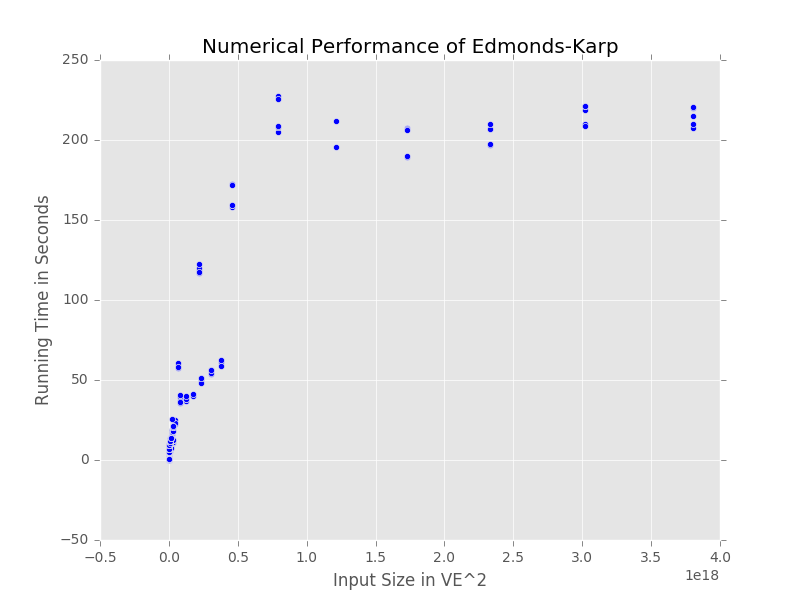
\includegraphics[width=0.5\textwidth]{images/ek-performance.png}
	\label{ek-performance}
\end{figure}

Figure \ref{ek-performance} plots the asymptotic performance $O(E^2V)$ against runtime. Like before, if this achieves linear or better performance then the asymptotic bound is upheld. Linear regression analysis of the data shows good statistical values of $r=.845,r^2=.714$. Discounting the tail end, this upholds the hypothesis that the data has a linear correlation. The tail end is sublinear therefore the empirical results agree with a runtime of $O(E^2V)$.

\subsubsection{Comparison Discussion}
Interestingly enough, performance results indicate that in practice Ford-Fulkerson outperformed Edmonds-Karp. Considering the trellis random graph input this is not surprising since edges within a layer are not interconnected which avoids some of the pathological performance issues of Ford-Fulkerson. A better comparison would include graphs where this behavior does occur. The other primary difference is that the variance of Ford-Fulkerson seemed to be higher than Edmonds-Karp.

\subsection{Computer Vision Datasets}
To analyze some real world performance of maximum flow algorithms computer vision data sets were used \cite{Verma:2012gs}. Although there were many data sets available, experiments were ran against the deconvolution data set with Ford-Fulkerson, Edmonds-Karp, NetworkX Edmonds-Karp, and NetworkX Push-Relabel \cite{networkx}. Experiments were conducted against two datasets, one called vision3 with $|E|=47872,|V|=2002,f=5668675$ and another called vision5 with $|E|=139600,|V|=2002,f=6849322$.

\begin{figure}[!ht]
	\caption{Deconvolution Performance}
	\label{vision}
	\begin{tabular}{c | c | c}
		Dataset & Algorithm & Runtime in Seconds\\
		\hline
		vision3 & FF & 26\\
		vision3 & EK & 2.6\\
		vision3 & NX-EK & 35\\
		vision3 & NX-PP & .55\\
		vision5 & FF & 109\\
		vision5 & EK & 13.3\\
	\end{tabular}
\end{figure}

The results of these experiments are in figure \ref{vision}. From these several conclusions can be drawn. First, on this dataset Ford-Fulkerson seems to perform much worse than Edmonds-Karp. Second, interestingly enough this Rust implementation of Edmonds-Karp for this project outperforms the NetworkX implementation by 10x. Finally, the Push Relabel maximum flow algorithm by Goldberg and Tarjan significantly outperforms all other algorithms which is consistent with its much better runtime asymptotic performance of $O(V^2E)$\cite{goldberg1988new}.

\section{Related Work}
	There is an abundant amount of work in this field some of which has already been mentioned. Maximum flow was first solved by Ford-Fulkerson in $O(Ef)$ time which was inconvenient since $f$ was unknown before the algorithm start\cite{Ford:1956vc}. This motivated the Edmonds-Karp algorithm which attained a runtime guarantee independent of the maximum flow $O(VE^2)$\cite{Edmonds:1972ht}. Although better, since $E=O(V^2)$ the runtime in terms of $V$ for a dense graph could approach $O(V^5)$ which is expensive. Although not discussed, Dinic's blocking flow algorithm followed shortly after which iterated on the shortest paths idea of using Breadth First Search to improve the running time to $O(V^2E)$\cite{Dinic:lsM40ti7}. This was further improved using dynamic trees to $O(EV\log V)$. The algorithm in most wide use today (as in NetworkX) is Push-relabel with runtime $O(V^2E)$\cite{goldberg1988new}. Most recently the flow problem has been solved in $O(VE)$ time by using Orlin's algorithm and the KRT algorithm\cite{orlin2013max}.

\section{Conclusion}
Through this report several goals are accomplished. First, the historical motivation for solving maximum flow is explored. Second, the correctness of both Ford-Fulkerson and Edmonds-Karp is shown in finding the maximal flow if there is one. Third, the asymptotic runtime behavior of these is analyzed. Fourth, experimental results show that the Rust implementation achieves the appropriate runtime and outperforms the implementation in the Python library NetworkX. Additionally, performance tests were done using computer vision datasets. Finally, Ford-Fulkerson and Edmonds-Karp are discussed in the context of other common and more advanced maximum flow algorithms.

\section{Resources}
In the course of learning about these algorithms the following sources were very helpful: \cite{cornell-ek},\cite{umass-ek}. Additionally, I used integration tests from Comp 572 at Hong Kong University to check correctness (in addition to many of my own tests)\cite{UstProject}.

\bibliographystyle{abbrv}
\bibliography{references}

%\balancecolumns 

\end{document}
